\documentclass{article}
\usepackage[utf8]{inputenc}
\usepackage{fancyhdr}
\usepackage{lastpage}
\usepackage{graphicx}
\usepackage{hyperref}
\usepackage{natbib}
\usepackage{amsmath,amstext}
\bibliographystyle{aasjournal}
\usepackage{pythonhighlight}
\usepackage{float}

\pagestyle{fancy}
\usepackage[margin=1in]{geometry}
\headwidth = 6.5in

\fancyhf{}
\headheight = 0.6in
\topmargin = -0.5in
\newcommand{\version}{1.0}

\lhead{
\includegraphics[height=0.5in]{./images/SPHEREx_logo.png}}
\chead{\large\spherex\ \vspace{1pt}{Test/Cal Control Software User Guide}}
\rhead{Version \version, 07-12-2021}
\footskip = 25pt
\cfoot{Page \thepage\ of \pageref{LastPage}}

\newcommand{\eps}{e$^{-}$ s$^{-1}$}

\newcommand{\spherex}{SPHEREx}

\begin{document}
	\begin{center}
		{\Large\bf SPHEREx Test and Calibration Control and Archive Software: User Guide}
		\vskip 0.25in
		{\large\bf Version: \version}
		\vskip 0.25in
		Sam Condon \texttt{scondon@caltech.edu} \\
		Marco Viero \texttt{mviero@caltech.edu} 
		\vskip 0.125in
	\end{center}
	
\section{Introduction and Setup}

The SPHEREx Test and Calibration Control and Archive Software provides a set of graphical user interface based tools allowing a user to interface with the suite of spectral and focus calibration instrumentation to specify automated measurement runs or manually control instruments in a measurement setup. This document provides a practical guide on how to use this GUI toolset in the SPHEREx test and calibration lab.

To run the most recent version of the GUI, navigate to the \textbf{SPHEREx-Test-Cal} folder located on the desktop of the b111-lab Lenovo laptop and double click the SpectralCalControl\_dev\_version.sh file after following the hardware setup instructions found in Appendix \ref{HW Setup Appendix}. 

Once the executable has started running, you should see two windows appear that are similar to what is seen in figure \ref{Main GUI}. One window is titled the \emph{Housekeeping Window} while the other is the \emph{Control Window}. As can be readily inferred from these titles, the \emph{Control Window} can be used to control lab instrumentation and set up automated measurement runs, while the \emph{Housekeeping Window} displays live time-streams of continuously sampled data.

\begin{figure}[H]
\label{Main GUI}
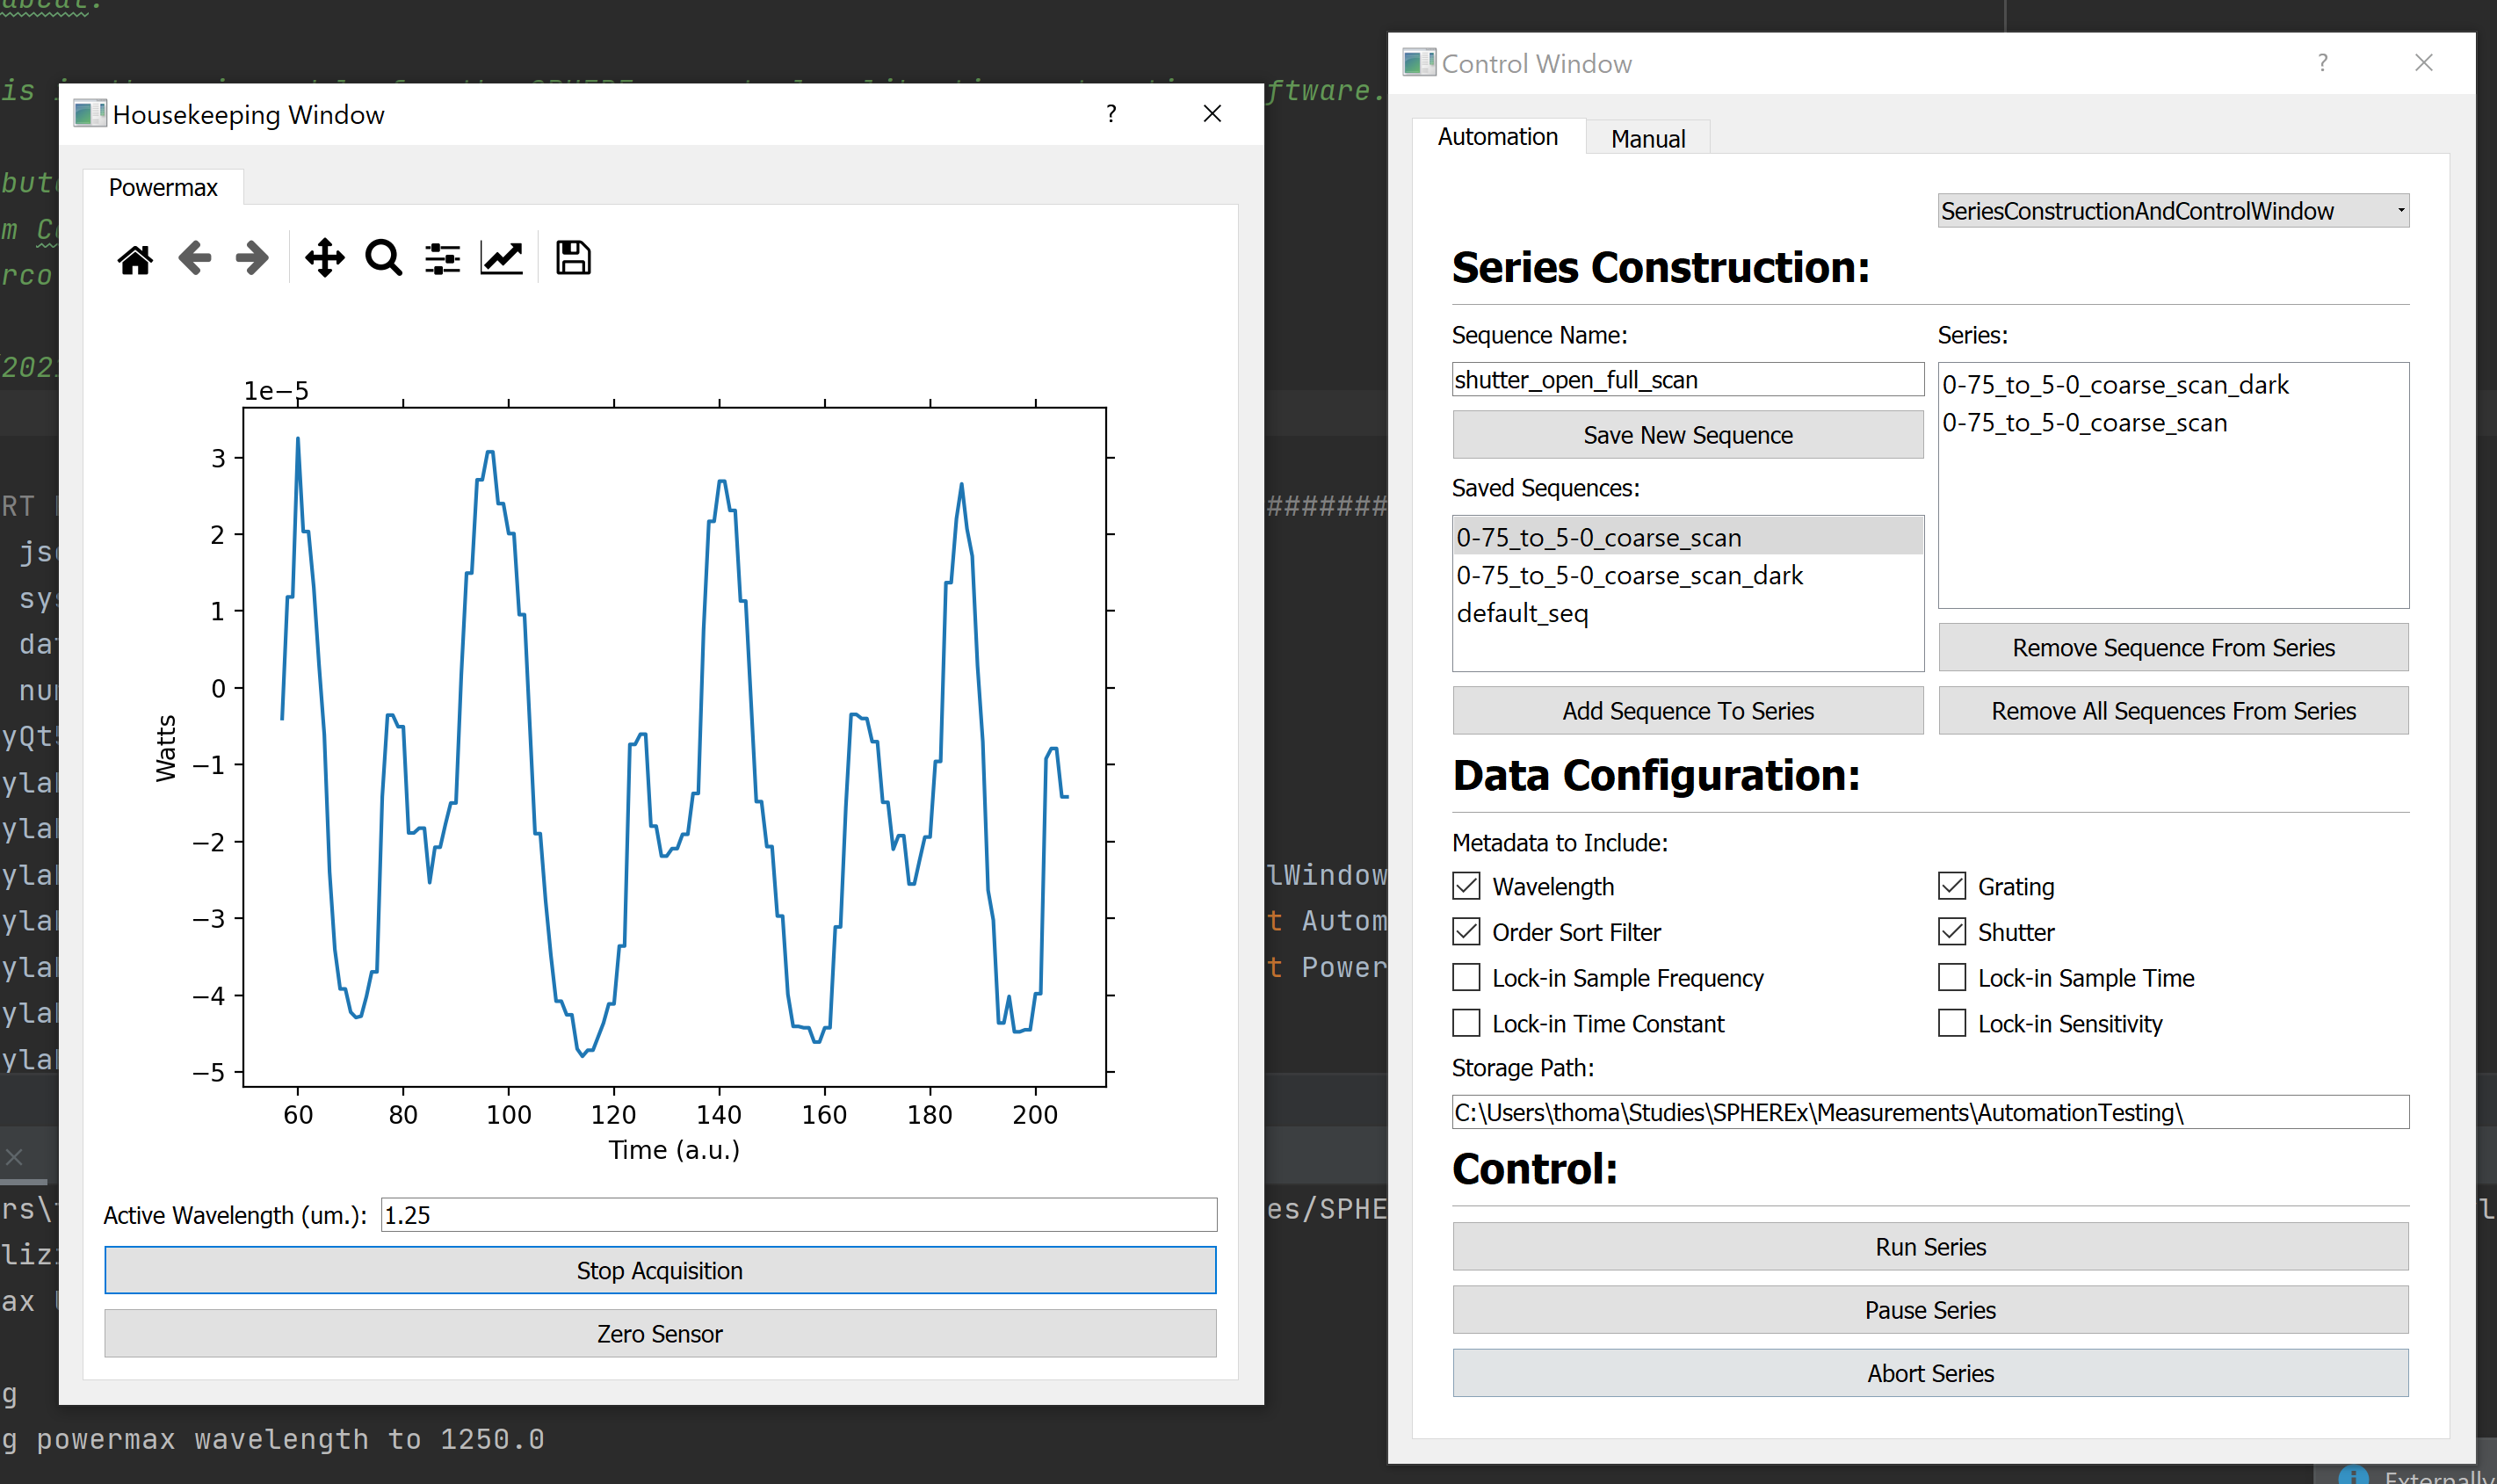
\includegraphics[width=\textwidth]{./images/MainGUIViews.png}
\caption{SPHEREx Test and Calibration Control and Archive GUI Main Windows: This figure shows the \emph{Housekeeping} and \emph{Control} windows which form the two main windows in version \version of the control software. Upon starting up the software, these windows should pop up. However, the plot seen in the \emph{Housekeeping Window} will be blank as only time-streams taken during the current session will be plotted.}	
\end{figure}

\section{Control Window}

As mentioned above, the \emph{Control Window} can be used to manually control instruments in a measurement setup or run entire automated measurement runs. Automation and manual control is divided into two tabs within the \emph{Control Window}. The highlight shown in Figure \ref{Automation Window Tabs Highlighted} shows where these tabs can be selected.   

\begin{figure}[H]
\label{Automation Window Tabs Highlighted}
\centering
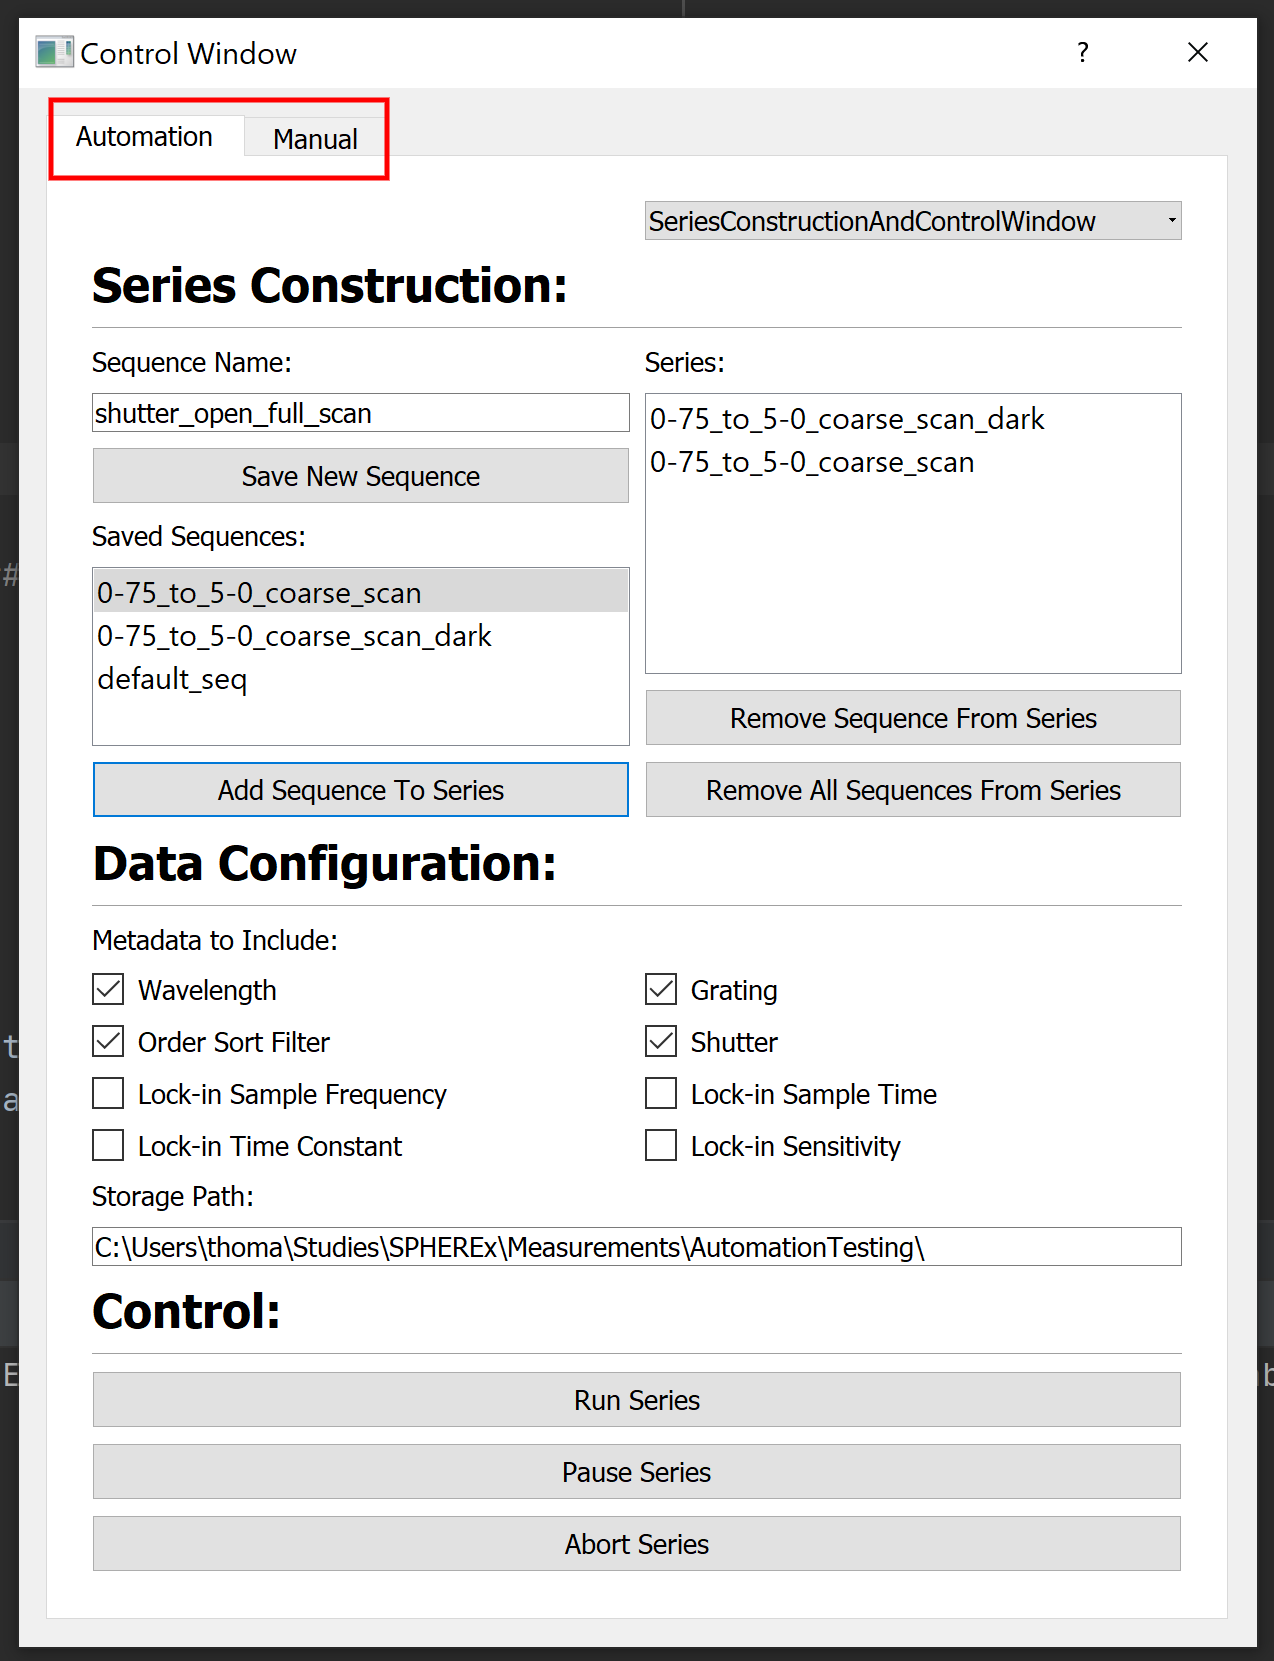
\includegraphics[width=0.7\linewidth]{./images/AutomationWindow_TabsHighlighted.png}
\caption{Control window with Automation and Manual tabs highlighted.}
\end{figure}

\subsection{Automation Tab}

Within the \emph{Control Window}, the \emph{Automation Tab} is used to setup and control entire automated measurement runs. The building blocks of an automation run are coined the \emph{Sequence} and the \emph{Series}. These terms are defined below:

\begin{enumerate}
	\item \textbf{Sequence}: A set of parameters specifying automated measurement actions to take and metadata to include in the final data package.
	\item \textbf{Series}: A collection of sequences. Used to specify an entire automation run.
\end{enumerate}

\subsection{Manual Tab}

\section{Time Stream Displays}
	
\section{Instruments Supported}
	
\appendix
\section{Hardware Setup} \label{HW Setup Appendix}	
	
\end{document}